\documentclass{article}
\usepackage{amsmath}
\usepackage{titlesec}
\usepackage{graphicx}
\usepackage[margin=1in]{geometry}
\usepackage{hyperref}
\usepackage{amssymb}
\usepackage{subfigure}

% Title, date, and author
\title{Project 3}
\author{Your Name, Collaborator's Name}
\date{\today}

\titleformat{\section}
  {\normalfont\normalsize\bfseries} % Format: font style, size, and weight
  {\thesection}{1em} % Label format and spacing
  {}
  \renewcommand{\thesubsection}{\thesection.\alph{subsection}}

\titleformat{\subsection}
  {\normalfont\small\bfseries} % Format: font style, size, and weight
  {\thesubsection}{1em} % Label format and spacing
  {}
\titleformat{\subsubsection}
  {\normalfont\small\bfseries} % Format: font style, size, and weight
  {\thesubsubsection}{1em} % Label format and spacing
  {}

\begin{document}
\begin{titlepage}
    \centering
    \vspace*{1in}
    
    {\Huge\bfseries Project 3\par}
    \vspace{1.5cm}
    {\Large \today\par}
    \vspace{1.5cm}
    {\Large\itshape Antonio Pampalone 23586519 \\ Giuseppe Pisante 23610012\\ Martina Raffaelli 23616907 \par}
    
    \vfill
    
\includegraphics[width=0.3\textwidth]{FAU-Logo.png}\par\vspace{1cm} % Adjust the width as needed
   
\end{titlepage}

\newpage
\small

\section*{\Large Task 3.0:}
To draw a sketch of the finite-volume discretization domain, it is important to first decide on the type of mesh and variable arrangement. For this task, we opted for a Cartesian mesh, as the domain's geometry is relatively simple and does not require the flexibility of unstructured grids. We chose a staggered arrangement for the variables, where pressure is stored at the center of the control volumes, and the velocity components $u$ and $v$ are located on the faces. This approach helps reduce pressure oscillations and improves the coupling between velocity and pressure, which is particularly beneficial when using the SIMPLE method. Additionally, we adopted a cell-centered storage scheme because it aligns naturally with the flux computation across control volume faces, ensuring consistency and simplicity in the discretization process.
The sketch is reported below:
\begin{figure}[h!]
  \centering
  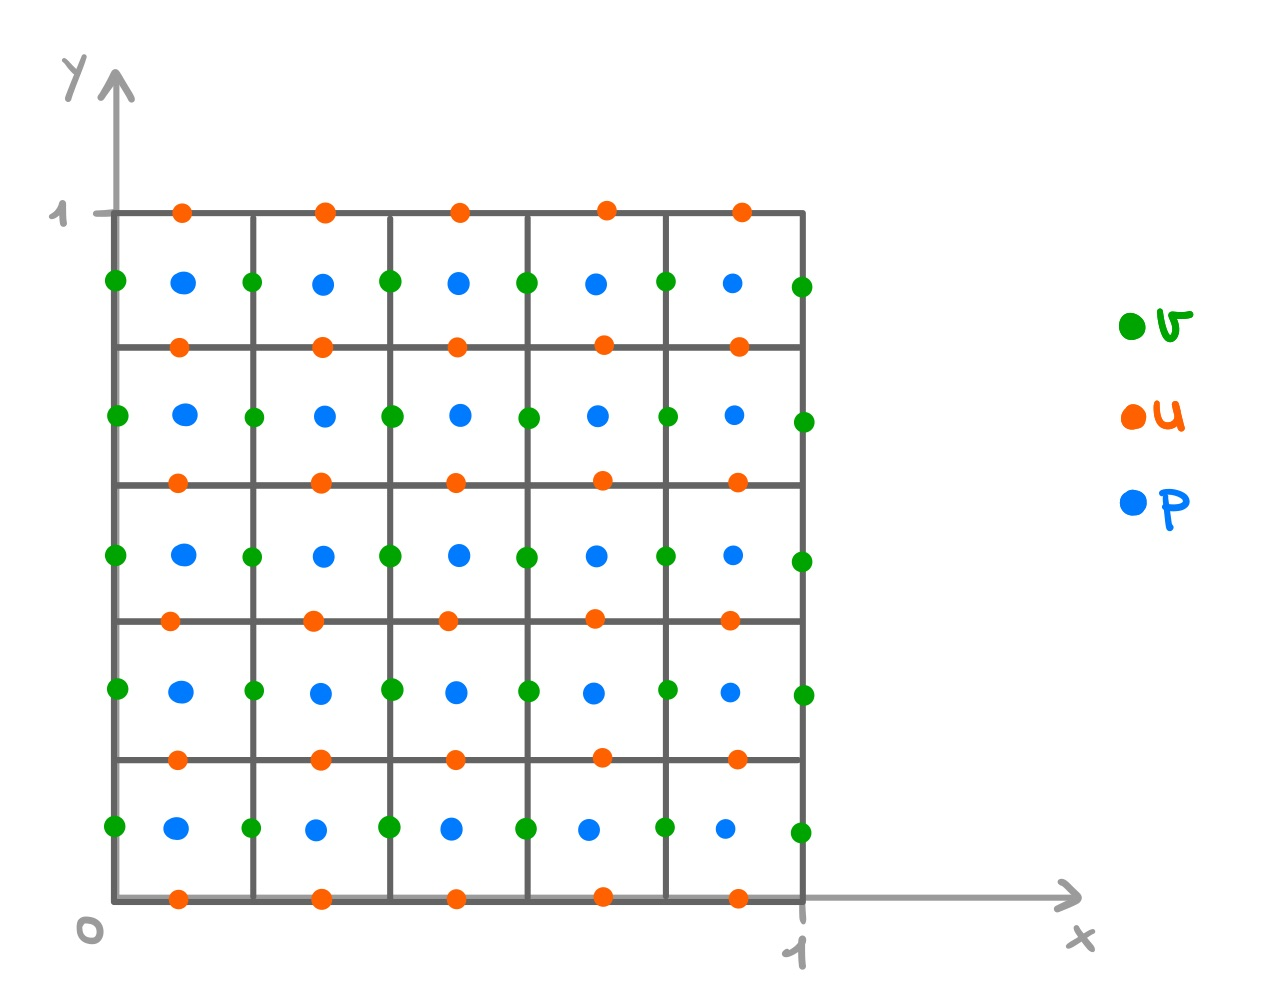
\includegraphics[width=0.5\textwidth]{staggered_grid.jpg}
  \caption{Finite-volume discretization of the domain}
\end{figure}
The yellow line highlights the wall nodes, on which we are going to impose the following boundary conditions:
\begin{itemize}
    \item $v = 0$ on all the walls,
    \item $u = 1$ on the lid,
    \item $u = 0$ on the rest of the walls,
    \item $\frac{\partial p}{\partial n} = 0$ on all the walls.
\end{itemize}
With those boundary conditions we are able to enforce: the motion of the fluid in the proximity of the lid, the no-slip condition on the walls, and the zero-gradient normal condition for the pressure (impermeability of the walls).
In particular we can specify the boundary conditions for the pressure on the single walls as follows:
\begin{itemize}
    \item $\frac{\partial p}{\partial x} = 0$ on right and left walls,
    \item $\frac{\partial p}{\partial y} = 0$ on top and bottom walls.
\end{itemize}

It is important to notice that to set properly the boundary conditions, we need to use interpolation since for some boundary conditions we don't have the variable we need to impose the condition on (for example the $v$ velocity on the top wall is not available, while it is on the left and right walls, where we are going to set it directly).


\section*{\Large Task 3.1:}

Since we are going to implement the SIMPLE method, we included in the formulation of the momentum equations the partial derivatives of the velocities in time. This was done because including the time derivative provides a more robust and stable approach to solving the problem. Additionally, it introduces a natural damping effect that facilitates the iterative process by preventing excessive corrections at each step, thereby avoiding divergence or slow convergence.
The starting point for deriving the finite-volume formulation of the x- and y-momentum equations are the following equations:
\begin{align}
  \frac{\partial u}{\partial t} + \frac{\partial u^2}{\partial x} + \frac{\partial uv}{\partial y} &= -\frac{\partial p}{\partial x} + \frac{1}{Re} \left( \frac{\partial^2 u}{\partial x^2} + \frac{\partial^2 u}{\partial y^2} \right) \\
  \frac{\partial v}{\partial t} + \frac{\partial uv}{\partial x} + \frac{\partial v^2}{\partial y} &= -\frac{\partial p}{\partial y} + \frac{1}{Re} \left( \frac{\partial^2 v}{\partial x^2} + \frac{\partial^2 v}{\partial y^2} \right).
\end{align}

We first focus on the x-momentum equation and then we perform an analogous procedure for y-momentum equation.
To discretize the x-momentum equation, we start by integrating it over the control volume and rearranging the terms as follows:
\begin{equation*}
  \int_{V}\frac{\partial u}{\partial t} + \int_{V} \frac{\partial}{\partial x} (u^2 - \frac{1}{Re} \frac{\partial u}{\partial x}) dV + \int_{V} \frac{\partial}{\partial y} (uv - \frac{1}{Re} \frac{\partial u}{\partial y}) = - \int_{V} \frac{\partial p}{\partial x} dV .
\end{equation*}
Notice that for simplicity and clearness we will consider the terms with $*$ apex as the values at time step $n+1$ and the terms without $*$ as the values at time step $n$.

Now we focus on one term at a time.

\subsubsection*{Discretization of the time component}
The integral of the transient term over the control volume is approximated by considering the average value of $\frac{\partial u}{\partial t}$ within the volume, then we approximate the derivative using a forward finite difference scheme.
The steps are reported below:
\begin{equation} \label{time_discretization}
  \int_V \frac{\partial u}{\partial t} \,dV = \frac{\overline{\partial u}}{\partial t} \Delta V \approx \frac{\partial u}{\partial t} \Delta V = \frac{u_{i,j}^{*} - u_{i,j}}{\Delta t} \Delta V = \frac{u_{i,j}^{*} - u_{i,j}}{\Delta t} \Delta x \Delta y
\end{equation}

\subsubsection*{Discretization of the pressure component}
Since we don't know the pressure distribution inside the control volumes, we need to perform an approxiamtion taking into account that we only know the pressure values at the cell centers.
\begin{equation} \label{pressure_discretization}
\begin{aligned}
  \int_{V} \frac{\partial p}{\partial x} dV &= \overline{\frac{\partial p}{\partial x}} \Delta V 
  \approx \frac{\partial p}{\partial x} \Delta V 
  = \frac{p_{e}^{*} - p_{w}^{*}}{\Delta x} \Delta x \Delta y 
  = \Delta y (p_{e}^{*} - p_{w}^{*})
\end{aligned}
\end{equation}
First we assume that the pressure gradient is constant inside the control volume, then we approximate $\frac{\partial p}{\partial x}$ as the difference between the pressure at east side and on the west side. We multiply this difference by the volume of the control volume to obtain the integral.

\subsection*{discretization of the first convection-diffusion term}
We first apply the divergence theorem to the first term, in order to transform the volume integral into a surface integral, and then we split the integral over the whole surface into two contributions, one for the east surface and one for the west surface of the control volume:
\begin{equation} \label{discr_1}
  \int_{V} \frac{\partial}{\partial x} (u^2 - \frac{1}{Re} \frac{\partial u}{\partial x}) dV = \int_{S} (u^2 - \frac{1}{Re} \frac{\partial u}{\partial x}) \mathbf{n} dS = \int_{S_{e}} (u^2 - \frac{1}{Re} \frac{\partial u}{\partial x}) \mathbf{n} dS + \int_{S_{w}} (u^2 - \frac{1}{Re} \frac{\partial u}{\partial x}) \mathbf{n} dS
\end{equation}

This leads to:
\begin{equation*}
  u_e^* u_e^* \Delta y - u_w^* u_w^* \Delta y - \frac{1}{Re} \left( \frac{u_e^* - u_c^*}{\Delta x} - \frac{u_c^* - u_w^*}{\Delta x}\right) \Delta y
\end{equation*}
Where $u_c^*$ is the velocity at the center of the staggered control volume used for solving the x-momentum equation.

Now we perform linearization since we have quadratic terms in our formulation. In particular we are linearizing the quadratic terms in this way: $u_e^* u_e^* \approx u_e u_e^*$ and the same for west, north and south terms so that the only unknowns are the ones with the $*$ apex.
\begin{equation*}
  u_e u_e^* \Delta y - u_w u_w^* \Delta y - \frac{1}{Re} \left( \frac{u_e^* - u_c^*}{\Delta x} - \frac{u_c^* - u_w^*}{\Delta x}\right) \Delta y.
\end{equation*}

Then we perform interpolation in order to compute the $u^*$ values at east, west, north and south positions:
\begin{equation*}
  u_e^* = \frac{u_{i,j+1}^* + u_{i,j}^*}{2}, \quad u_w^* = \frac{u_{i,j}^* + u_{i,j-1}^*}{2}, \quad u_n^* = \frac{u_{i+1,j}^* + u_{i,j}^*}{2}, \quad u_s^* = \frac{u_{i,j}^* + u_{i-1,j}^*}{2}.
\end{equation*}
Notice that analogous approximations hold for $u_e$, $u_w$, $u_n$ and $u_s$, but for simplicity we are not expliciting them since they are known.

We substitute these interpolated values in the equation, we simplify $\Delta x$ and $\Delta y$ since we are considering the grid to be equi-spaced in x and y, and we obtain:
\begin{equation}
  u_e \frac{u_{i,j+1}^* + u_{i,j}^*}{2} \Delta y - u_w \frac{u_{i,j}^* + u_{i,j-1}^*}{2} \Delta y - \frac{1}{Re} \left( \frac{u_{i,j+1}^* + u_{i,j}^*}{2} - u_{i,j}^* - u_{i,j}^* - \frac{u_{i,j-1}^* + u_{i,j}^*}{2}\right).
\end{equation}

\subsection*{Discretization of the first convection-diffusion term}
For the second term we proceed in the same way as before and we obtain:
\begin{equation*}
   \int_{V} \frac{\partial}{\partial y} (uv - \frac{1}{Re} \frac{\partial u}{\partial y}) dV = \int_{S} (uv - \frac{1}{Re} \frac{\partial u}{\partial y}) \mathbf{n} dS = \int_{S_{e}} (uv - \frac{1}{Re} \frac{\partial u}{\partial y}) \mathbf{n} dS + \int_{S_w} (uv - \frac{1}{Re} \frac{\partial u}{\partial y}) \mathbf{n} dS.
\end{equation*}

This leads to:
\begin{equation*}
  u_n^* v_n^* \Delta y - u_s^* v_s^* \Delta y - \frac{1}{Re} \left( \frac{u_n^* - u_c^*}{\Delta y} - \frac{u_c^* - u_s^*}{\Delta y}\right) \Delta x.
\end{equation*}

At this point we still need to linearize the terms that include a multiplication between a $u$ term and a $v$ term. We perform the linearization by approximating $v^*$ as $v$ since here we are solving the x-momentum equation and we are interested in the $u$ velocity (for the y-momentum equation we are treating these two terms in the opposite way).
Then we perform interpolation, simplification between $\Delta x$ and $\Delta y$ and we get:
\begin{equation}
  v_n \frac{u_{i+1,j}^* + u_{i,j}^*}{2} \Delta y - v_s \frac{u_{i,j}^* + u_{i-1,j}^*}{2} \Delta y - \frac{1}{Re} \left( \frac{u_{i+1,j}^* - u_{i,j}^*}{2} - u_{i,j}^* - u_{i,j}^* - \frac{u_{i,j}^* - u_{i-1,j}^*}{2}\right).
\end{equation}

\subsection*{Final discretized x-momentum equation}
As the last step we sum up all the terms we computed before and we collect the terms with the same unknowns:
\begin{gather*}
    u_{i,j}^* \left(\frac{u_e \Delta y}{2} - \frac{u_w \Delta y}{2} + \frac{2}{Re} + \frac{v_e \Delta y}{2} - \frac{v_w \Delta y}{2} + \frac{\Delta x \Delta y}{dt} \right) \\
    + u_{i+1,j}^* \left(- \frac{1}{2 Re} + \frac{v_n \Delta y}{2} \right) \\
    + u_{i-1,j}^* \left(- \frac{1}{2 Re} - \frac{v_s \Delta y}{2} \right) \\
    + u_{i,j+1}^* \left(- \frac{u_e \Delta y}{2} - \frac{1}{2 Re} \right) \\
    + u_{i,j-1}^* \left(- \frac{u_w \Delta y}{2} - \frac{1}{2 Re} \right) \\
    = u_{i,j} \frac{ \Delta x \Delta y}{dt} + \Delta y (p_{e}^* - p_{w}^*)
\end{gather*}
This equation is the discretized x-momentum equation for the staggered grid.

\subsection*{Discretization of the y-momentum equation}
We perform the same procedure for the y-momentum equation and we get:
\begin{gather*}
    v_{i,j}^* \left(\frac{v_n \Delta x}{2} - \frac{v_s \Delta x}{2} + \frac{2}{Re} + \frac{u_n \Delta x}{2} - \frac{u_s \Delta x}{2} + \frac{\Delta x \Delta y}{dt} \right) \\
    + v_{i+1,j}^* \left(\frac{v_n \Delta x}{2} - \frac{1}{2 Re} \right) \\
    + v_{i-1,j}^* \left(- \frac{v_s \Delta x}{2} - \frac{1}{2 Re} \right) \\
    + v_{i,j+1}^* \left(- \frac{1}{2 Re} + \frac{u_e \Delta x}{2} \right) \\
    + v_{i,j-1}^* \left(- \frac{1}{2 Re} - \frac{u_w \Delta x}{2} \right) \\
    = v_{i,j} \frac{ \Delta x \Delta y}{dt} + \Delta x (p_{n}^* - p_{s}^*)
\end{gather*}
Notice that to explicit the values $v_n$, $v_s$, $v_w$ and $v_e$ we need to perform the following interpolations:
\begin{equation*}
  v_n^* = \frac{v_{i+1,j}^* + v_{i,j}^*}{2}, \quad v_s = \frac{v_{i,j}^* + v_{i-1,j}^*}{2}, \quad v_e = \frac{v_{i,j+1}^* + v_{i,j}^*}{2}, \quad v_w = \frac{v_{i,j}^* + v_{i,j-1}^*}{2}.
\end{equation*}

From the picture reported below we can see where we are going to solve the three equations.
\begin{figure}[h!]
  \centering
  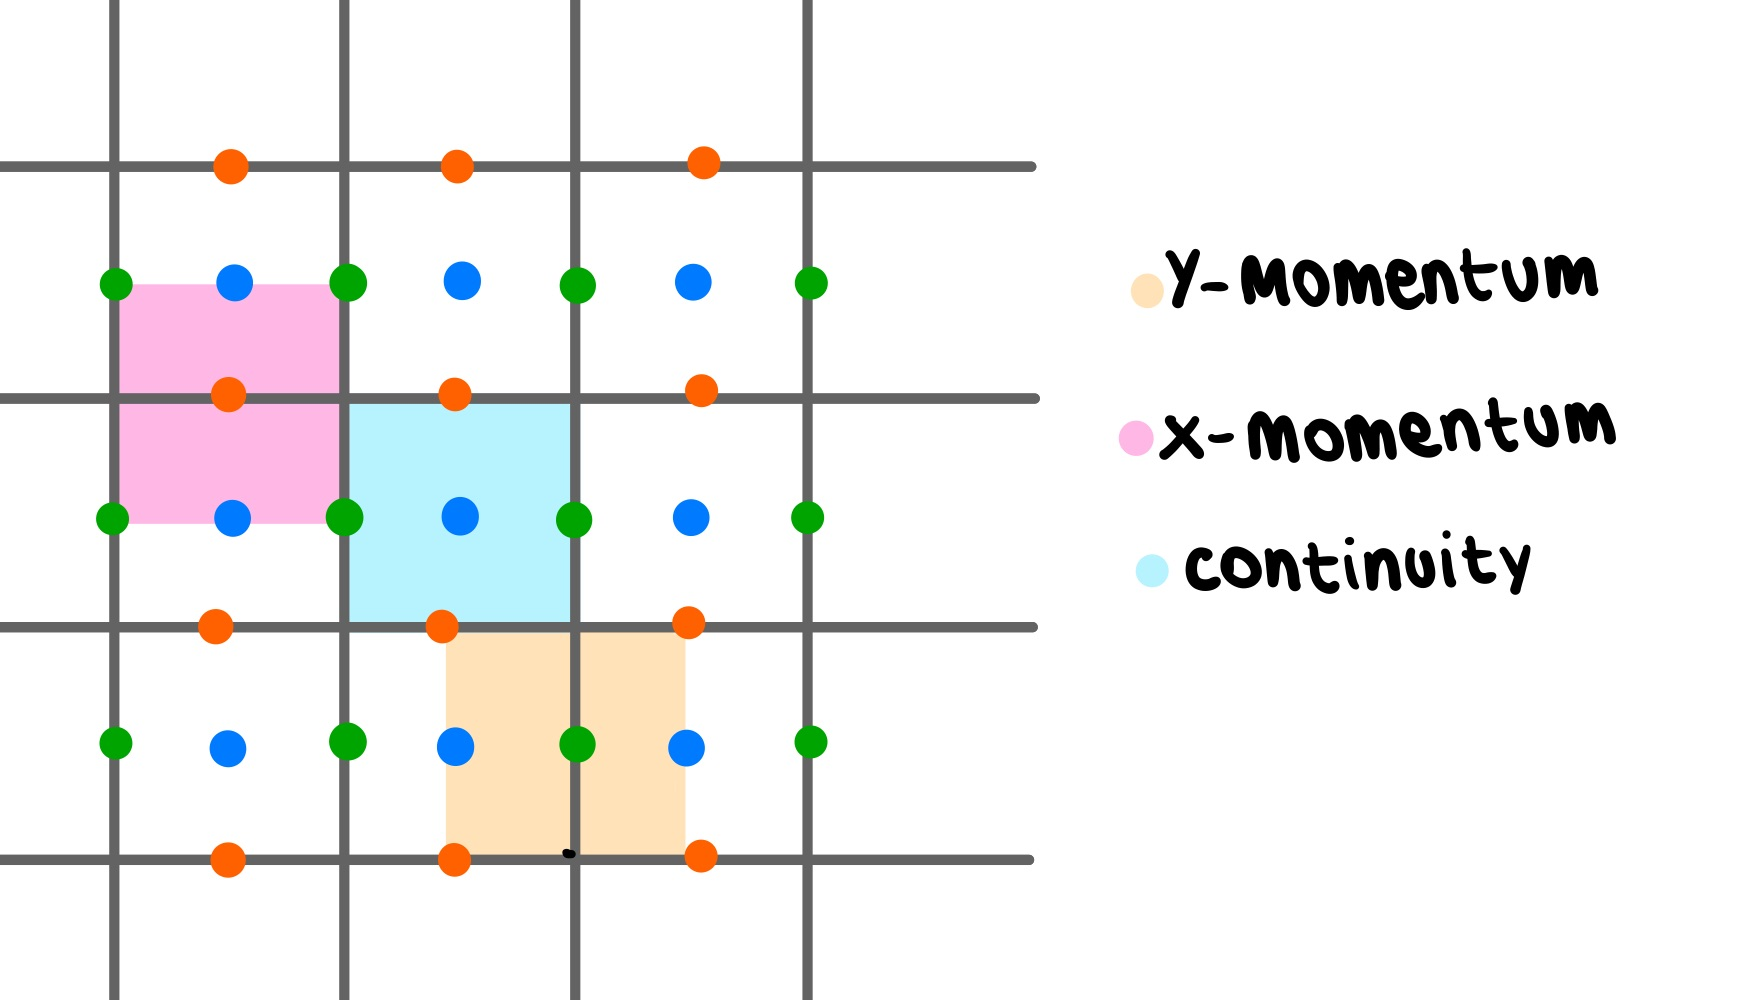
\includegraphics[width=0.5\textwidth]{equations_grid.jpg}
  \caption{Different equations for the staggered grid}
  \label{equations_grid}
\end{figure}
For the x-momentum equation we are going to use as reference cell the pink one where $u$ velocity is stored in the center.
For this equation we need to compute $v_n$ and $v_s$ by interpolating the values of $v$ at the edges of the reference cell:
\begin{equation*}
  v_n = \frac{v_{i+1,j} + v_{i,j}}{2}, \quad v_s = \frac{v_{i,j} + v_{i-1,j}}{2}.
\end{equation*}

For the y-momentum equation we take as reference cell the orange one, where $v$ velocity is stored in the center and we need to compute the values of $u_e$ and $u_w$ by interpolating the values of $u$ at the edges of the reference cell:
\begin{equation*}
  u_e = \frac{u_{i,j+1} + u_{i,j}}{2}, \quad u_w = \frac{u_{i,j} + u_{i,j-1}}{2}.
\end{equation*}
  

\newpage
\section*{\Large Task 3.2:}
Our knowledge on the SIMPLE method came from the course slides and was deepend by the book \cite{Book} at page 597.
\subsubsection*{1) Initialization}
We set an initial guess for velocities ($u^*$ and $p^*$) and pressure ($p^*$) fields and we ensure that the values are consistent with the boundary conditions.
We also set relaxation parameters ($\alpha_p$ and $\alpha_u$) to control the convergence of the solution.

\subsubsection*{2) Prediction step}
In this step we solve the momentum equations to compute the intermediate velocities $u^*$ and $v^*$.
In particular, for the x-momentum equation we have the following formula to solve implicitly:
\begin{equation}
  a_{c}u_{c}^*=\sum_{nb}a_{nb}u_{nb}^*+b_{u}-\frac{\partial p^{*}}{\partial x}
\end{equation}
where $a_{c}$, $a_{nb}$ and $b_{u}$ are the coefficients that derive from the discretization equation.
This equation is solved considering the pink reference cell of the picture \ref{equations_grid}.

For y-momentum equation we have the analogue formula (which is going to be solved considering the orange reference cell):
\begin{equation}
  a_{c}v_{c}^*=\sum_{nb}a_{nb}v_{nb}^*+b_{u}-\frac{\partial p^{*}}{\partial y}.
\end{equation}

We solve these equations for all the cells in order to obtain the predicted velocities $u^*$ and $v^*$.

\subsubsection*{3) Correction step}
This step is necessary to ensure that the continuity equation is satisfied, so we are solving it in the blue reference cells. 
We start by deriving the pressure correction equation from the continuity equation:
\begin{equation}
  \frac{\partial u}{\partial x} + \frac{\partial v}{\partial y} = 0
\end{equation}
and then we substitute the corrected velocities $u = u^* + u'$ and $v = v^* + v'$ in the equation, where $u'$ and $v'$ are the corrections to the velocities due to pressure correction. 
Substituting them into the equation and exploiting the linearity property of the partial derivatives, we get:
\begin{equation}
  \frac{\partial u^*}{\partial x} + \frac{\partial v^*}{\partial y} + \frac{\partial u'}{\partial x} + \frac{\partial v'}{\partial y} = 0
\end{equation}

For the momentum equations, the velocity corrections $u'$ and $v'$ are proportional to the pressure correction $p'$, as follows:
\begin{equation}
  u' = -\frac{\Delta x}{a_P} \frac{\partial p'}{\partial x}, \quad v' = -\frac{\Delta y}{a_P} \frac{\partial p'}{\partial y}.
\end{equation}
where $a_P$ is the coefficient of the discretized momentum equation.

Then we substitute the velocity corrections in the continuity equation and we obtain the pressure correction equation:
\begin{equation}
  \frac{\partial}{\partial x}\left(-\frac{\Delta x}{a_P}\frac{\partial p'}{\partial x}\right) + \frac{\partial}{\partial y}\left(-\frac{\Delta y}{a_P}\frac{\partial p'}{\partial y}\right) = -\left(\frac{\partial u^*}{\partial x} + \frac{\partial v^*}{\partial y}\right)
\end{equation}

Then we integrated over the control volume and apply the divergence theorem to convert the volume integrals into surface integrals, and we approximate the gradients at the faces of the control volume using central differences.
Then we assemble the  resulting terms into a discretized Poisson equation for $p'$,where the source term is the divergence of the predicted velocity field $u^*$ and $v^*$, and we get:
\begin{equation}
  a_P p'_P = \sum_{nb} a_{nb} p_{nb} + b_p
\end{equation} 
where $p'_P$ is the pressure correction at the cell center, $p'_{nb}$ are the pressure corrections at the neighboring cells (east, west, north, south), $a_P$ and $a_{nb}$ are the coefficients that derive from the discretization equation, and the source term is $b_p = \rho \left( \frac{u_E^* - u_W^*}{\Delta x} + \frac{v_N^* - v_S^*}{\Delta y} \right)$. 

This equation forms a system of linear equations that is solved using numerical methods (e.g., iterative solvers like Jacobi).


\subsubsection*{4) Update pressure and velocity fields}
We update the pressure field in order to ensure that the corrected velocity field satisfies the continuity equation. 
The update of the pressure field $p^{\nu +1}$ is calculated as:
\begin{equation}
  p^{\nu+1} = p^* + \alpha_p p'
\end{equation}
where $\alpha_p$ is the relaxation factor for pressure and it controls how much of the correction is applied.

Then we adjust the predicted velocities as follows:
\begin{equation}
  u^{\nu+1} = u^* - \frac{\Delta x}{a_P} \frac{\partial p'}{\partial x}, \quad v^{\nu+1} = v^* - \frac{\Delta y}{a_P} \frac{\partial p'}{\partial y}.
  \end{equation}
where the approximations for the partial derivatives of the pressure are: $\frac{\partial p'}{\partial x} = \frac{p'_{E} - p'_{W}}{\Delta x}$ and $\frac{\partial p'}{\partial y} = \frac{p'_{N} - p'_{S}}{\Delta y}$.

\subsubsection*{5) Convergence check}
At the end we evaluate convergence criteria for both velocity and pressure fields. We can use the following criteria:

\begin{itemize}
  \item Velocity u: $||u^{\nu+1} - u^*|| \leq \text{tolerance}$.
  \item Velocity v: $||v^{\nu+1} - v^*|| \leq \text{tolerance}$.
  \item Pressure: $||p^{\nu+1} - p^*|| \leq \text{tolerance}$.
\end{itemize}

If not converged, set $u^* = u^{\nu+1}$, $v* = v{\nu+1}$ and $p^* = p^{\nu+1}$ and repeat the process from step 2.

The method can be summarized in the following flow-chart:
\begin{figure}[h!]
  \centering
  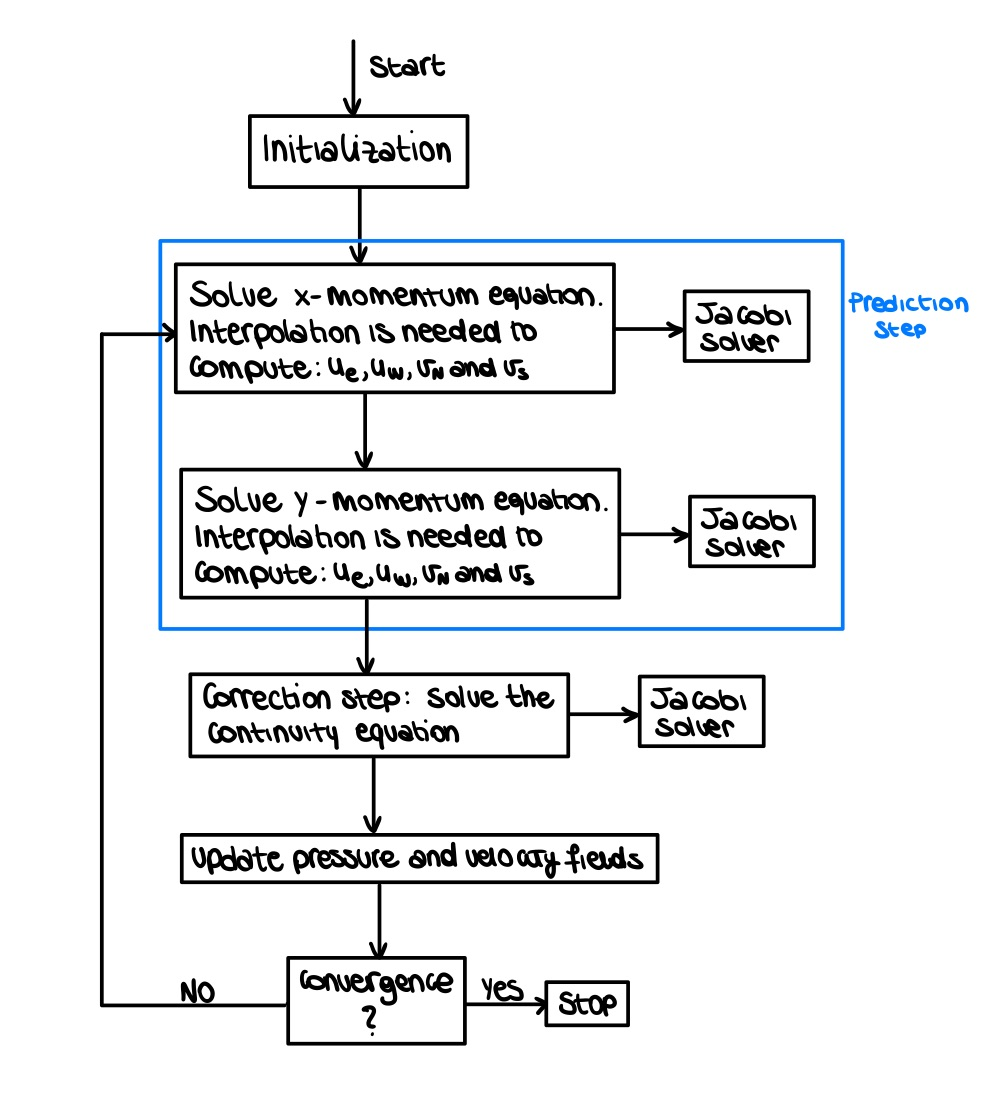
\includegraphics[width=0.5\textwidth]{graph.jpg}
  \caption{Flowchart of the method}
\end{figure}

\section*{\Large Task 3.3:}
The code is structured in two files, visible at the github repository \cite{GitHubRepo}. In the solver.py file the are 3 functions: solver, SimpleSolver and Jacobi solver. 
In particular, solver applies the simplesolver until convergence, whose tolerance is compared to the increment of the solutions of u, v and p of the previous iteration.
The SimpleSolver applies the simple iterattions and uses jacobi to solve the 3 systems in a sequrntial manner, as explained previously. The vectores of the system are unrolled in a colMajor fashion to allow to create such systems.
Finally, the tolerance for the whole study was set to 1e-4.
\section*{\Large Task 3.4:}
The velocities and pressure fields, the vorticity and the streamlines of the flow for a grid with 100 control volumes is reported below for the 3 Reynolds number required.
\begin{figure}[h!]
  \centering
  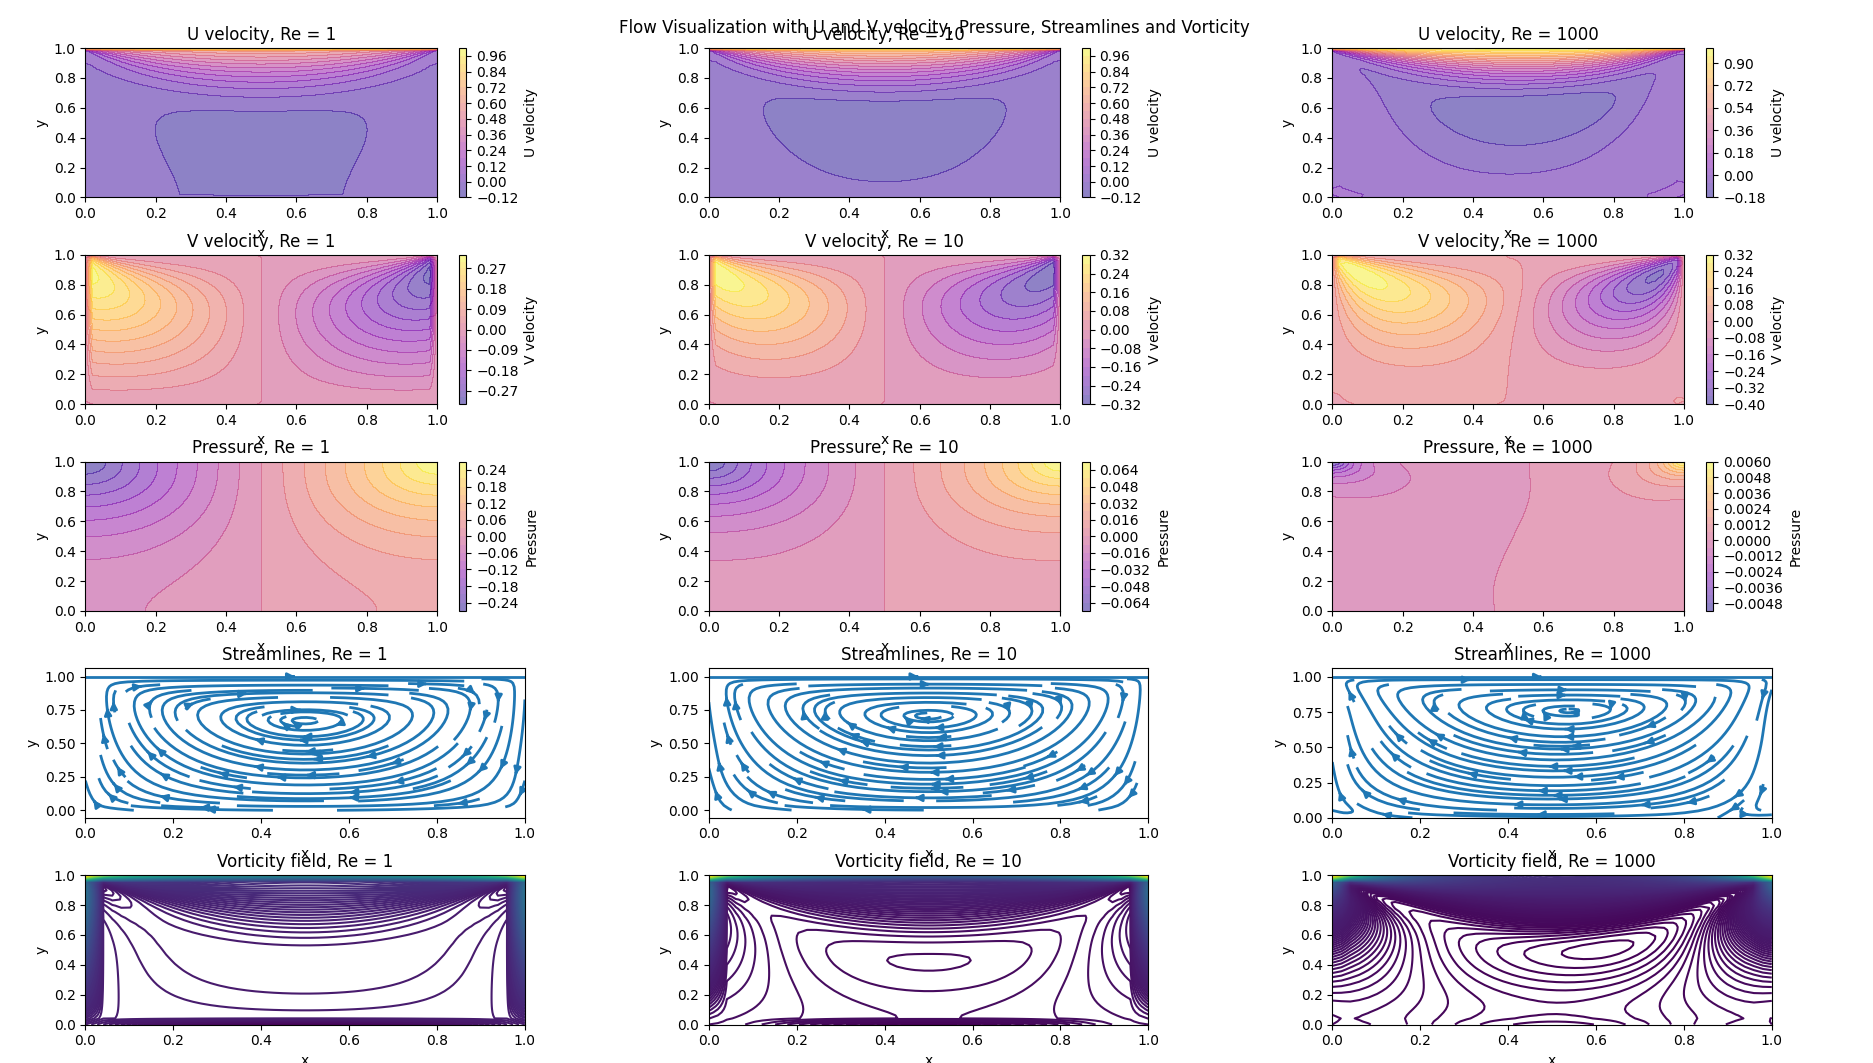
\includegraphics[width=0.7\textwidth]{Task4.png}
  \caption{Velocities and pressure fields, vorticity and streamlines for different Reynolds numbers}
\end{figure}

From such plots we can see that by increasing the Reynolds number the vortex center moves towards the right of the domain. In addition, The U-velocity field demonstrates predominant horizontal kinematics adjacent to the moving lid, 
characterized by progressively intensifying velocity gradients with increasing Reynolds number. The V-velocity field reveals a more intricate flow mechanism near lateral boundaries, with increasingly complex recirculatory patterns 
emerging at elevated $Re$. Pressure distributions maintain uniform symmetry at low Reynolds numbers, while higher $Re$ manifests more pronounced gradients concentrated in corner regions.
The vorticity field accentuates the growing dynamical complexity, exhibiting concentrated rotational intensities proximal to boundaries and exhibiting sharp gradient characteristics at $Re = 1000$.

\section*{\Large Task 3.5:}
From the following plots we can see some problems in the convergence of the y-momentum, which is unexpected since the discretization follows the same principles and the jacobi solver works the same way.
\begin{figure}[h!]
  \centering
  \begin{minipage}{0.32\textwidth}
    \centering
    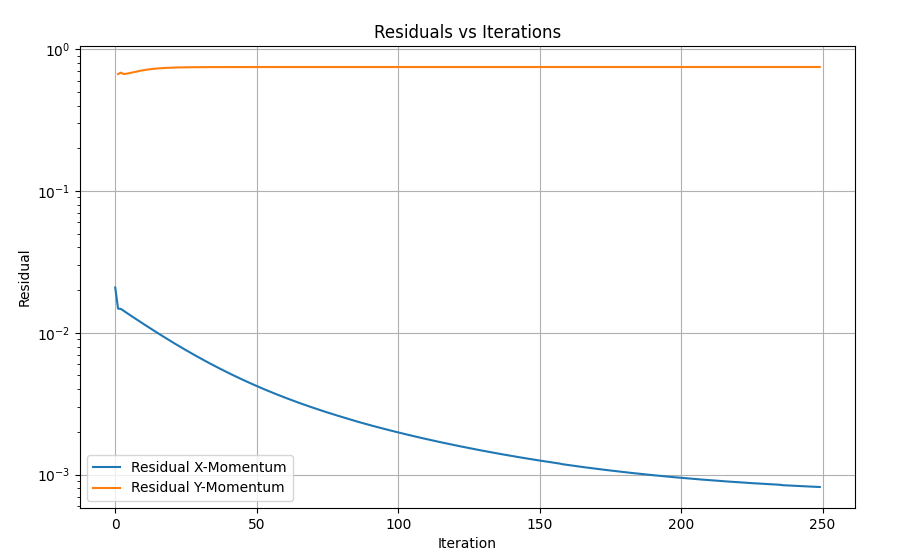
\includegraphics[width=\textwidth]{Residual Re 1.png}
    \caption{Re = 1}
  \end{minipage}
  \begin{minipage}{0.32\textwidth}
    \centering
    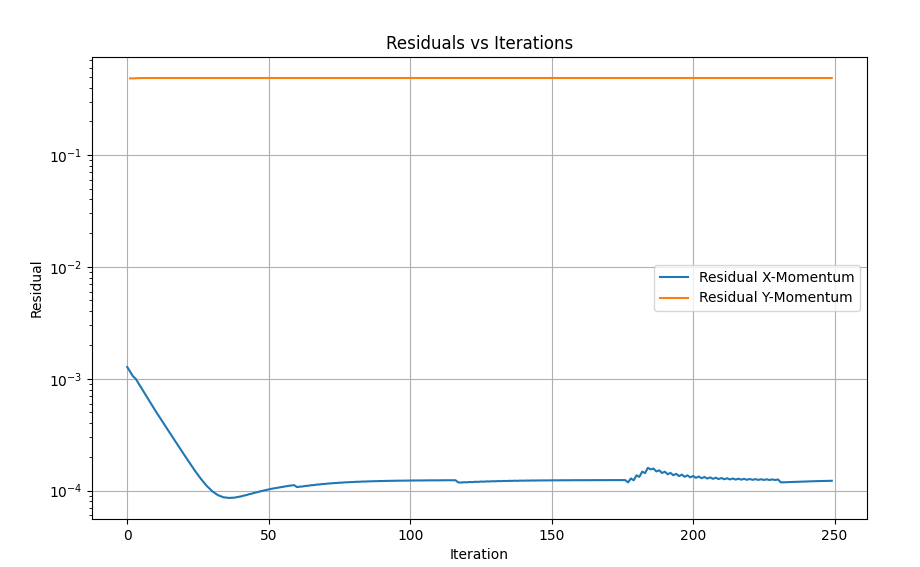
\includegraphics[width=\textwidth]{Residual Re 10.png}
    \caption{Re = 100}
  \end{minipage}
  \begin{minipage}{0.32\textwidth}
    \centering
    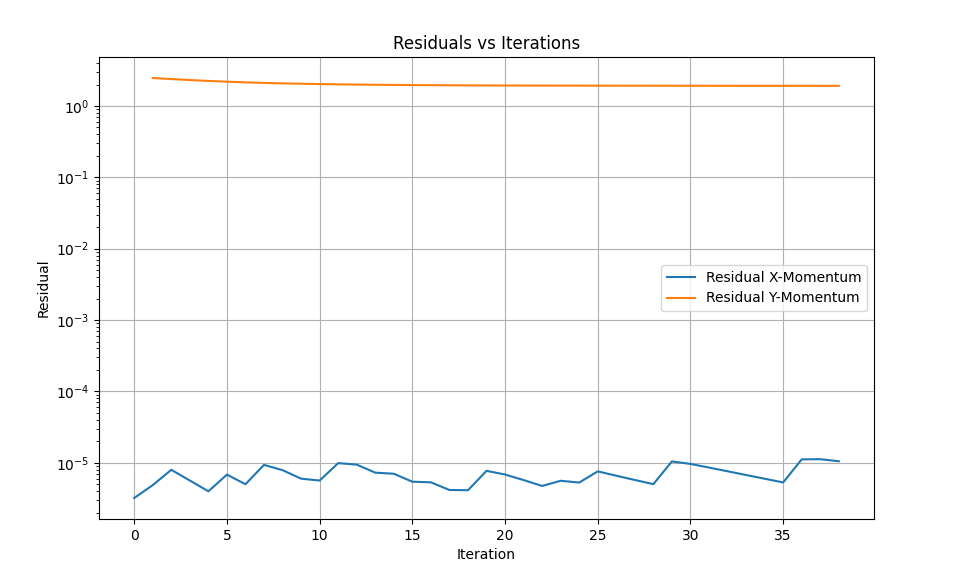
\includegraphics[width=\textwidth]{Residual Re 1000.png}
    \caption{Re = 1000}
  \end{minipage}
  \caption{Residuals for different Reynolds numbers}
\end{figure}

What is clear from the 3 pictures, looking only at the x-momentum, is that the residuals are decreasing, which is a good sign of convergence. This is more evident for bigger Reynolds numbers, which is coherent from what we expected in terms of stability.
In addition, it is possible to see that with a higher Reynolds number, the number of simple iterations is clearly lower.
\section*{\Large Task 3.6:}
The locations where chosen in order to try to show in the most complete way the gradient of the velocities and pressure. In particular, this was found in the center of the vortex, which as previously mentioned, was slightly de-centered towards the right part of the domain.
\begin{figure}[h!]
  \centering
  \begin{minipage}{0.49\textwidth}
    \centering
    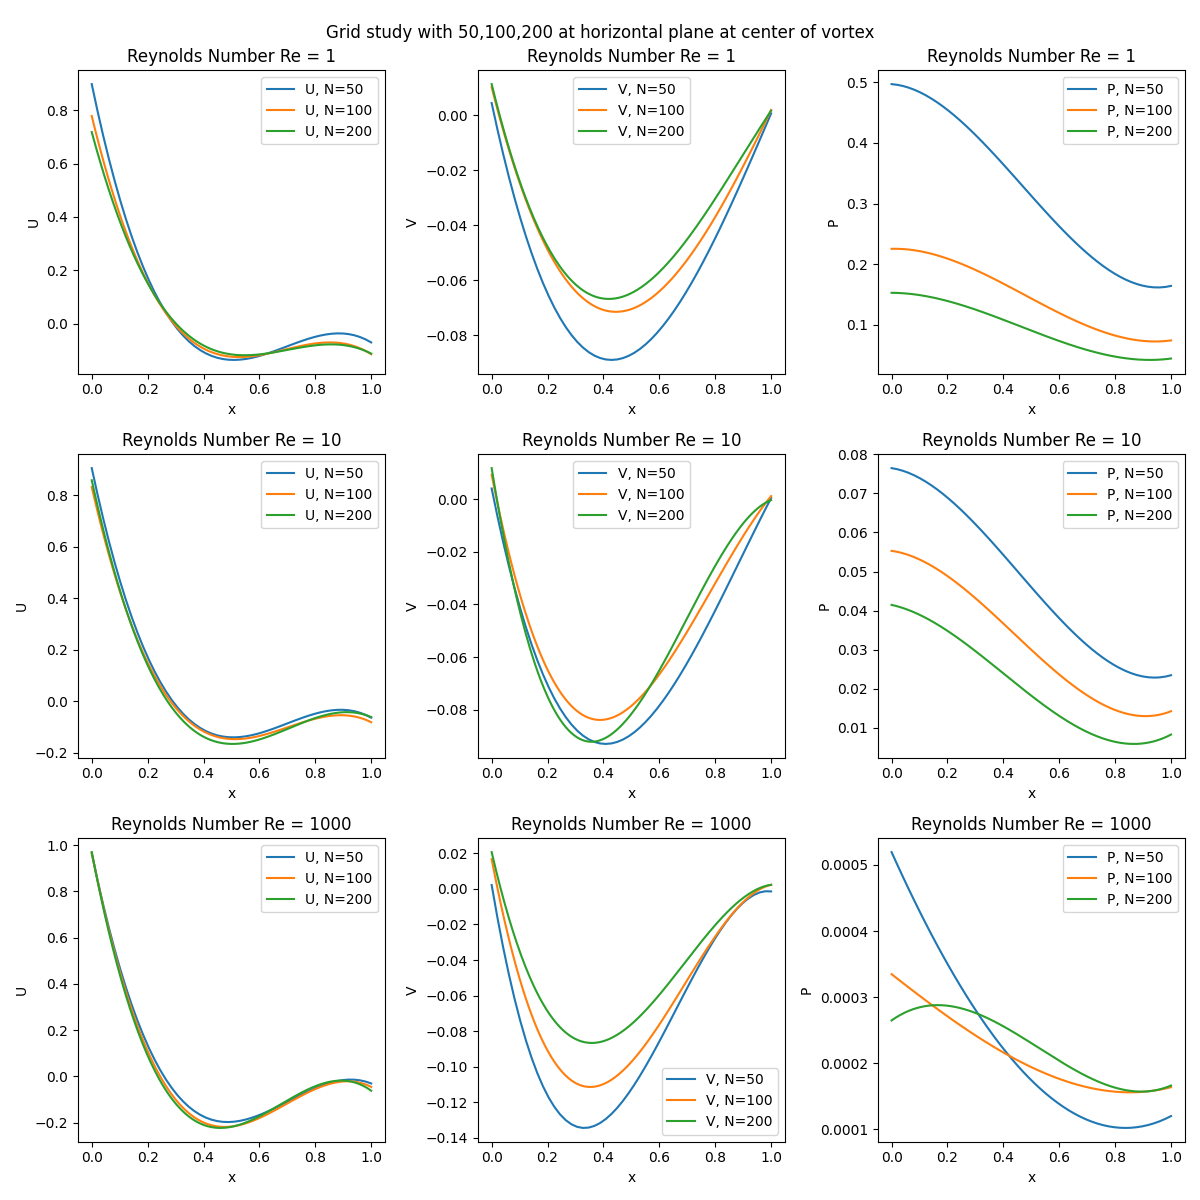
\includegraphics[width=\textwidth]{horizontal_plane.png}
    \caption{Horizontal projection}
  \end{minipage}
  \hfill
  \begin{minipage}{0.49\textwidth}
    \centering
    \includegraphics[width=\textwidth]{vertical_plane.png}
    \caption{Vertical projection}
  \end{minipage}
\end{figure}
It is clear that there is a slight difference in the solution of the 3 different domains. In particular, taking N=200 as the baseline, N=50 is the one further from it.
All the 3 options show that the minimum of u is in the vortex, as expected and the boundary conditions are also met. The same is for v and P, where the neumann conditions are not fully visible since in the code, in order to plot in the same domain, an interpolation was made to reduce the dimension of the pressure grid.
It is important to note that in some cases the plots look slightly different from one discretization to another, probably due to the stopping criteria used, which was based, as previously mentioned, on the error convergence and on a max iteration, to prevent the simulation to take too much time. This could be the reason why the pressure for Re=1000 has such a strange pattern with N=200.
\section*{\Large Task 3.7:}
Below are shown the error with the different Reynolds number.
\begin{figure}[h!]
  \centering
  \begin{minipage}{0.49\textwidth}
    \centering
    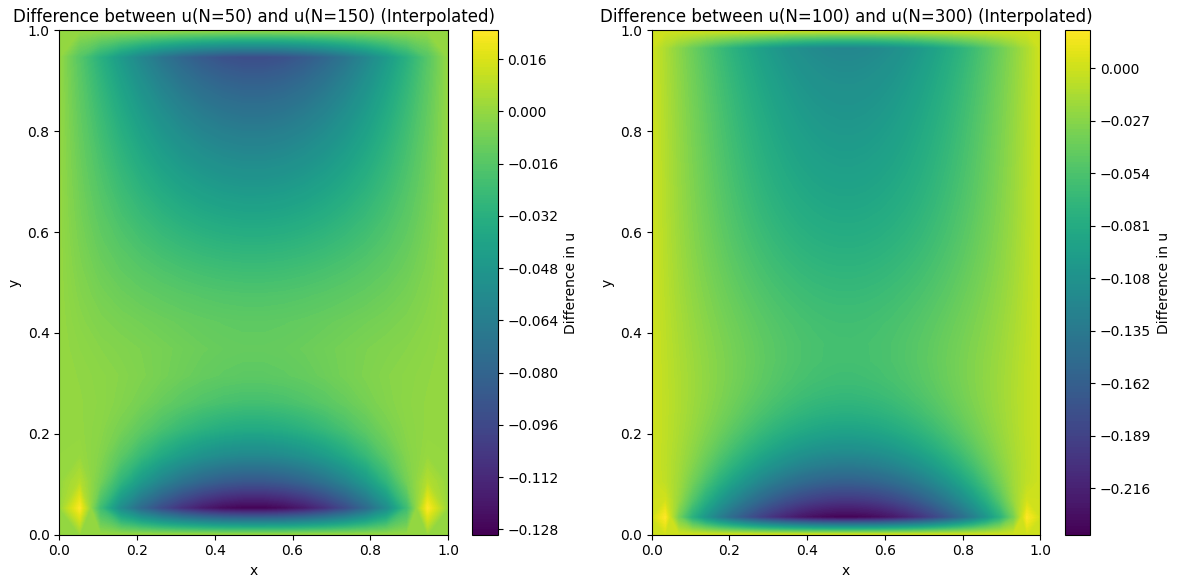
\includegraphics[width=\textwidth]{udiff1.png}
    \caption{Error for Reynolds = 1 on (u)}
  \end{minipage}
  \hfill
  \begin{minipage}{0.49\textwidth}
    \centering
    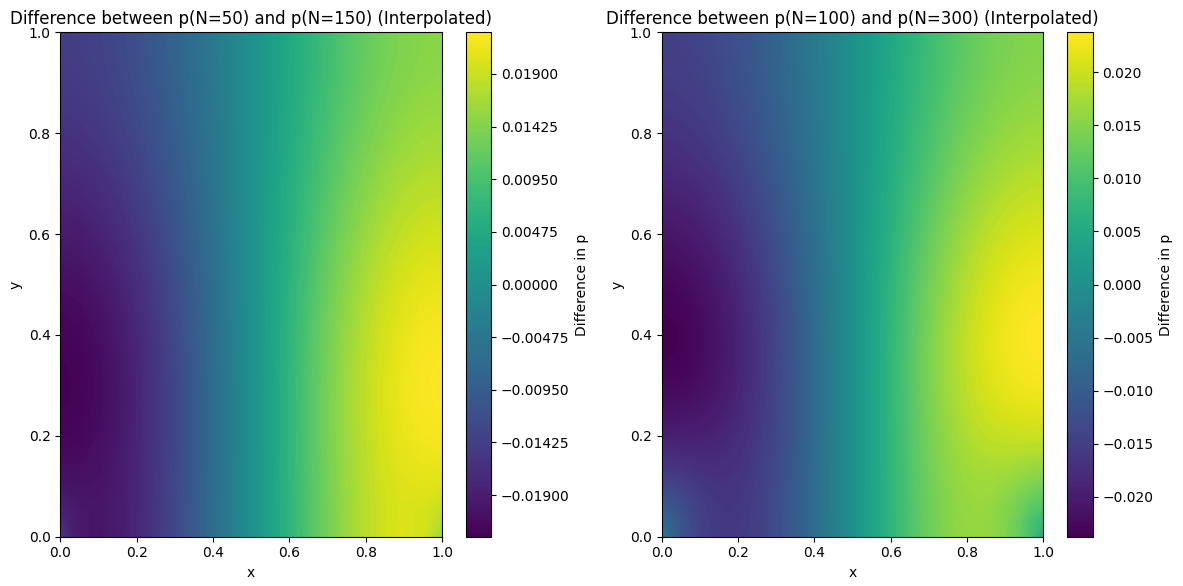
\includegraphics[width=\textwidth]{pdiff1.png}
    \caption{Error for Reynolds = 1 on (p)}
  \end{minipage}
\end{figure}
\begin{figure}[h!]
  \centering
  \begin{minipage}{0.49\textwidth}
    \centering
    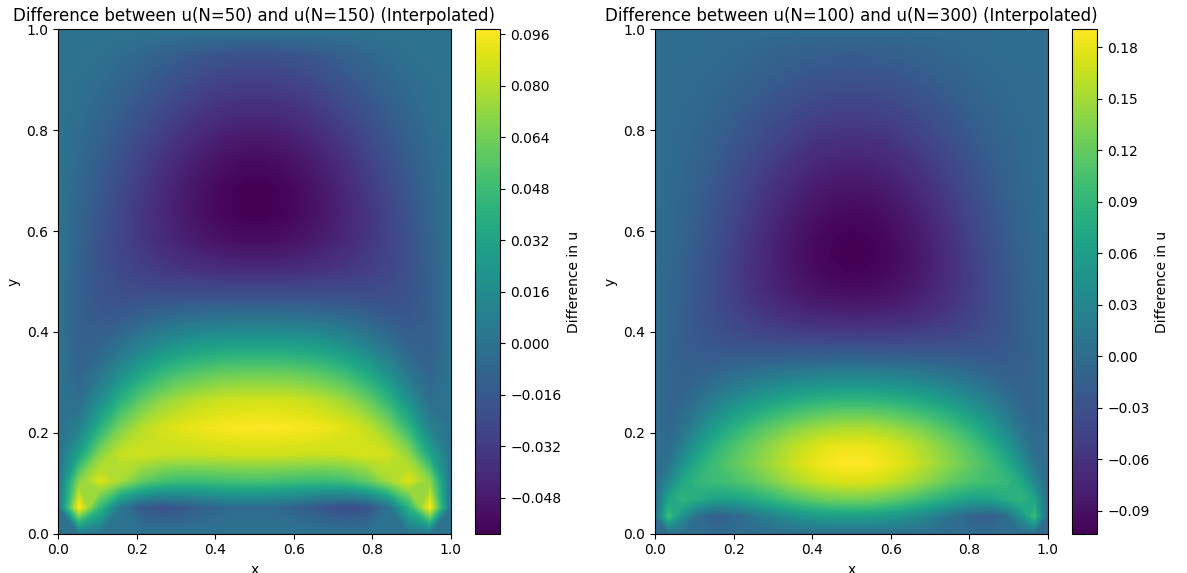
\includegraphics[width=\textwidth]{udiff100.png}
    \caption{Error for Reynolds = 100 on (u)}
  \end{minipage}
  \hfill
  \begin{minipage}{0.49\textwidth}
    \centering
    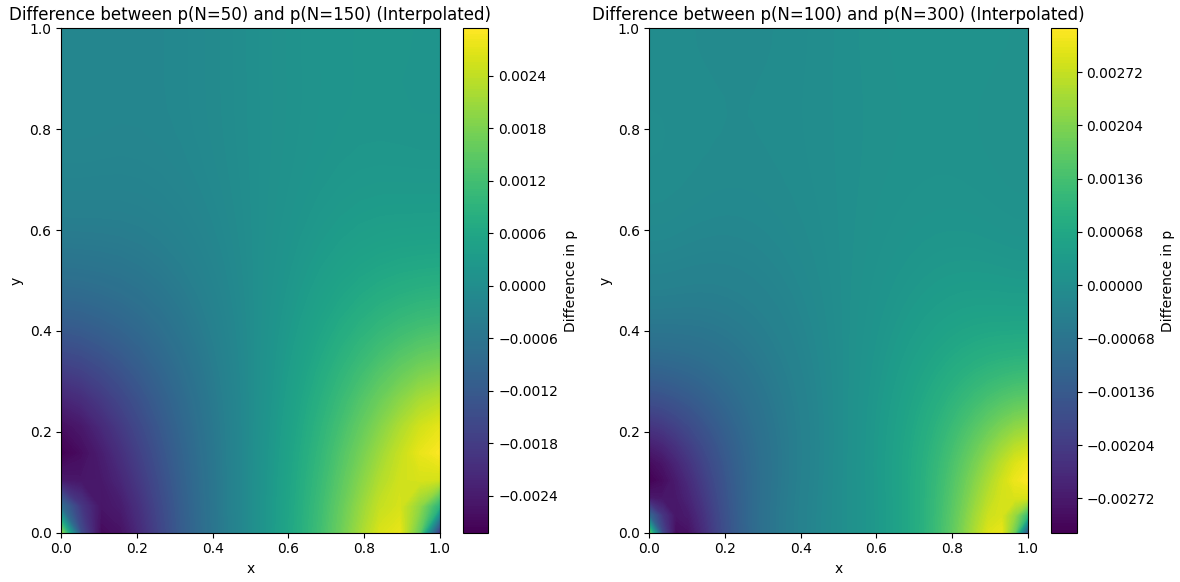
\includegraphics[width=\textwidth]{pdiff100.png}
    \caption{Error for Reynolds = 100 on (p)}
  \end{minipage}
\end{figure}
\begin{figure}[h!]
  \centering
  \begin{minipage}{0.49\textwidth}
    \centering
    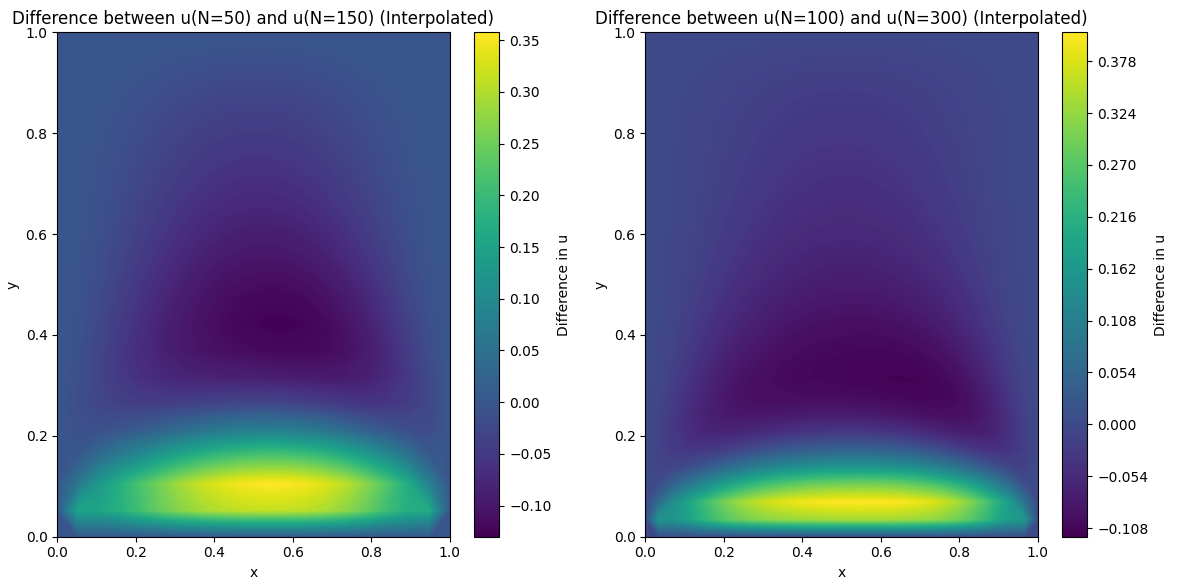
\includegraphics[width=\textwidth]{udiff1000.png}
    \caption{Error for Reynolds = 1000 on (u)}
  \end{minipage}
  \hfill
  \begin{minipage}{0.49\textwidth}
    \centering
    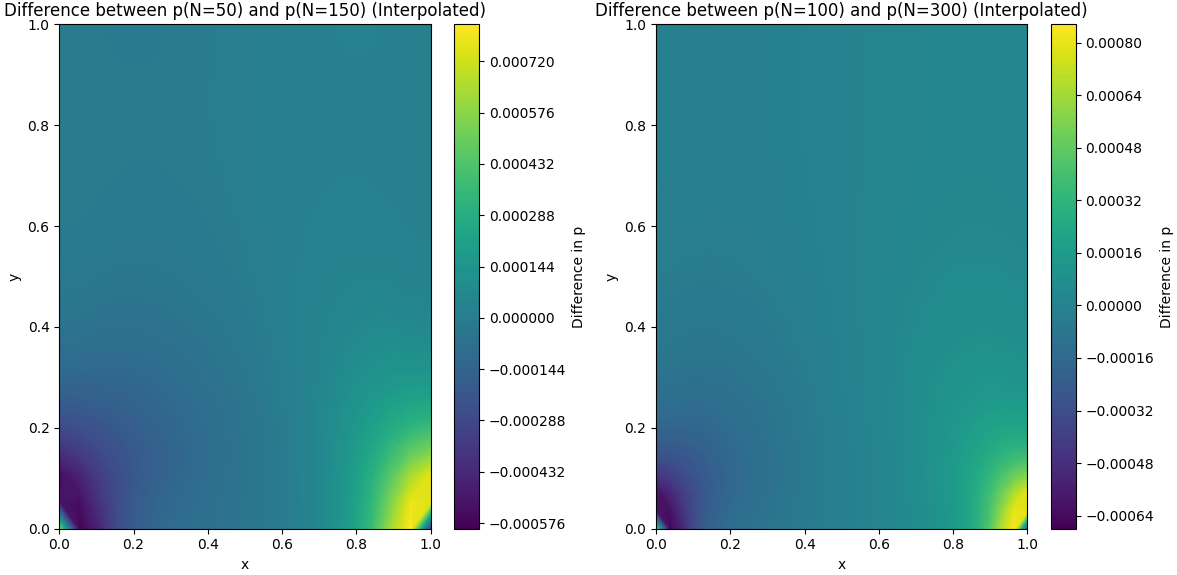
\includegraphics[width=\textwidth]{pdiff1000.png}
    \caption{Error for Reynolds = 1000 on (p)}
  \end{minipage}
\end{figure}

From the plots, it looks like the error is mostly relevant where the gradient is higher. In particular, this is very visible in the pressure field. 
In addition, the error is higher for lower Reynolds numbers, which is coherent with what we expected in terms of stability.

\newpage
\begin{thebibliography}{9}
    \bibitem{Book}
    \textit{The FVM in CFD},\\
    F.Moukalled, L.Mangani, M.Darwish. Springer, 2016.

    \bibitem{GitHubRepo}
    \textit{CFD Repository},\\
    Available at: \url{https://github.com/GiuseppePisante/CFD.git}
    
    \bibitem{GitHubCopilot}
    \textit{GitHub Copilot},\\
    GitHub. Available at: \url{https://github.com/features/copilot}
    \end{thebibliography}

\end{document}